\chapter{آزمایش‌ها، نتایج و تحلیل}
\label{ch:experiments}

در این فصل، معماری \lr{DuoDiT} در سناریوی تولید تصویر شرطی روی \lr{ImageNet-1K} ارزیابی می‌شود. هدف اصلی، سنجش این پرسش است که آیا افزودن یک شاخه دوم با وضوح توکنی بالاتر، در حالی که بدنه اصلی \lr{DiT-XL/2} منجمد باقی می‌ماند، می‌تواند کیفیت توزیعی و ادراکی تولید را با بودجه پارامتری کوچک بهبود دهد یا خیر. به همین منظور، نتایج \lr{DuoDiT} با \lr{DiT-XL/2}، \lr{LightningDiT} و \lr{FineDiffusion} مقایسه می‌شود \cite{2212.09748,Yao2025LightningDiT,Pan2024FineDiffusion}.

\section{پیکربندی آزمایش}
ارزیابی اصلی بر روی تولید شرطی \lr{ImageNet-1K} در وضوح $256 \times 256$ انجام شده است \cite{5206848,imagenet15russakovsky}. مطابق پروتکل \lr{FID-50K}، تعداد ۵۰٬۰۰۰ تصویر تولید می‌شود؛ برچسب هر نمونه به‌صورت یکنواخت از میان ۱۰۰۰ کلاس 
\lr{ImageNet}
 انتخاب می‌گردد و سپس کیفیت نمونه‌ها در برابر آمار مرجع 
\lr{ImageNet}
 محاسبه می‌شود. 
\subsection{جزئیات پیاده‌سازی}
مدل پایه در تمام آزمایش‌ها \lr{DiT-XL/2} است که شامل ۲۸ بلوک مبدل، بعد پنهان ۱۱۵۲ و ۱۶ سر توجه است. شاخه اصلی با اندازه پچ ۲ روی فضای نهان عمل می‌کند، در حالی که شاخه دوم \lr{DuoDiT} اندازه پچ ۱ دارد و بنابراین توکن‌های ریزدانه‌تری تولید می‌کند. بلوک خبره \lr{ViT} در شاخه دوم از وزن‌های از پیش آموزش‌دیده \lr{vit\_large\_patch16\_224} مقداردهی اولیه شده و برای تطبیق بعد ۱۰۲۴ این بلوک با بعد ۱۱۵۲ در \lr{DiT-XL/2}، پروجکشن‌های خطی ورودی و خروجی آموزش داده می‌شوند \cite{Dosovitskiy2020,wightman2019timm,2212.09748}.

تصاویر ورودی با برش مرکزی، وارونگی تصادفی افقی و نرمال‌سازی به بازه $[-1,1]$ پیش‌پردازش می‌شوند. سپس تصاویر با استفاده از رمزگذار \lr{sd-vae-ft-ema} به فضای نهان $32 \times 32 \times 4$ نگاشت شده و ضریب مقیاس \lr{0.18215} اعمال می‌شود \cite{9851474}. بهینه‌ساز \lr{AdamW} با نرخ یادگیری ثابت $10^{-4}$، اندازه دسته سراسری ۲۵۶، ضرایب $\beta_1=0.9$ و $\beta_2=0.999$ و وزن‌کاهی صفر استفاده شده است \cite{loshchilov2019adamw}. مدل \lr{DuoDiT-200} برای ۲۰۰ دوره آموزش داده شده و نسخه \lr{DuoDiT-57} به‌عنوان نقطه میانی آموزش نیز گزارش می‌شود.

برای پایداری آموزش، میانگین متحرک نمایی (\lr{EMA}) با ضریب فروپاشی \lr{0.9999} روی وزن‌های آموزش‌پذیر اعمال شده است \cite{Polyak1992EMA,ho2020ddpm}. در نمونه‌برداری، از \lr{DDPM} با ۲۵۰ گام و ضریب هدایت بدون طبقه‌بند \lr{CFG=1.5} استفاده شده است \cite{ho2020ddpm,ho2022classifierFreeGuidance}. احتمال حذف برچسب کلاس در آموزش برابر \lr{0.1} است تا نمونه‌برداری شرطی و غیرشرطی برای \lr{CFG} پشتیبانی شود. به بیان عملی، این مقدار حذف برچسب باعث می‌شود همان مدل در زمان نمونه‌برداری بتواند هم خروجی وابسته به کلاس و هم خروجی مستقل از کلاس را تولید کند؛ سپس \lr{CFG} اختلاف این دو خروجی را تقویت می‌کند تا نمونه نهایی به برچسب انتخاب‌شده نزدیک‌تر شود. مقدار \lr{CFG=1.5} به‌عنوان تنظیم میانه استفاده شده است، زیرا هدف ارزیابی فقط تولید نمونه‌های بسیار کلاس‌محور نیست، بلکه حفظ تعادل میان وفاداری شرطی، تنوع و کیفیت توزیعی نیز اهمیت دارد.

\begin{table}[htbp]
    \centering
    \caption[خلاصه تنظیمات آموزش و نمونه‌برداری]{خلاصه ابرپارامترها و تنظیمات مورد استفاده در آموزش و نمونه‌برداری \lr{DuoDiT}.}
    \label{tab:hyperparams}
    \begin{latin}
    \resizebox{\textwidth}{!}{%
    \begin{tabular}{llc}
        \hline
        \textbf{Category} & \textbf{Parameter} & \textbf{Value} \\
        \hline
        \multirow{7}{*}{Model} & Architecture & DiT-XL/2 \\
         & Transformer Depth & 28 \\
         & Hidden Dimension & 1152 \\
         & Attention Heads & 16 \\
         & MLP Ratio & 4.0 \\
         & Main Patch Size & 2 \\
         & Second Stream Patch Size & 1 \\
        \hline
        \multirow{9}{*}{Training} & Image Resolution & $256 \times 256$ \\
         & VAE & sd-vae-ft-ema \\
         & Diffusion Steps & 1000 \\
         & Optimizer & AdamW \\
         & Learning Rate & $1 \times 10^{-4}$ \\
         & Global Batch Size & 256 \\
         & Epochs & 200 \\
         & Seed & 0 \\
         & Label Dropout & 0.1 \\
        \hline
        \multirow{2}{*}{Sampling} & DDPM Steps & 250 \\
         & CFG Scale & 1.5 \\
        \hline
    \end{tabular}%
    }
    \end{latin}
\end{table}

\section{نتایج کمی}
جدول \ref{tab:main_metrics} مقایسه اصلی مدل‌ها را نشان می‌دهد. \lr{LightningDiT} بهترین مقدار \lr{FID} گزارش‌شده را دارد، اما \lr{DuoDiT-200} در \lr{KID} و \lr{LPIPS-Mean} بهترین عملکرد را میان مدل‌های مقایسه‌شده ثبت می‌کند. این نتیجه نشان می‌دهد شاخه دوم \lr{DuoDiT} بیشتر از آنکه صرفاً یک تنظیم پارامتری سطحی باشد، می‌تواند در کیفیت ادراکی و شباهت توزیعی مبتنی بر \lr{KID} اثر بگذارد.

\begin{table}[htbp]
    \centering
    \caption[مقایسه کمی اصلی]{مقایسه کمی اصلی میان مدل‌های ارزیابی‌شده. معیارهای \lr{FID}، \lr{KID} و \lr{LPIPS-Mean} همگی کمتر-بهتر هستند.}
    \label{tab:main_metrics}
    \begin{latin}
    \footnotesize
    \resizebox{\textwidth}{!}{%
    \begin{tabular}{lcccc}
        \hline
        \textbf{Model} & \textbf{FID} ($\downarrow$) & \textbf{KID} ($\downarrow$) & \textbf{LPIPS-Mean} ($\downarrow$) & \textbf{Params/Trainable (M)} \\
        \hline
        DiT-XL/2 \cite{2212.09748} & 2.270$^\dagger$ & 0.0023 & 0.7209 & 675.00$^\dagger$ \\
        LightningDiT \cite{Yao2025LightningDiT} & \textbf{1.350}$^\dagger$ & 0.0016 & 0.7232 & 675.00$^\dagger$ \\
        FineDiffusion \cite{Pan2024FineDiffusion} & 9.674 & 0.0093 & 0.7802 & 685.64 / 12.15 \\
        \hline
        DuoDiT-57 & 4.95 & 0.0069 & 0.7175 & 690.39 / 17.95 \\
        DuoDiT-200 & 2.219 & \textbf{0.0014} & \textbf{0.7162} & 690.39 / 17.95 \\
        \hline
    \end{tabular}%
    }
    \end{latin}
    \begin{minipage}{0.96\linewidth}
        \footnotesize
        مقادیر دارای $^\dagger$ از گزارش رسمی مقاله یا پروژه متناظر گرفته شده‌اند. \lr{DuoDiT-57} و \lr{DuoDiT-200} معماری یکسان دارند و تفاوت آن‌ها در تعداد دوره‌های آموزش است.
    \end{minipage}
\end{table}

جدول \ref{tab:classwise_fid_aggregate} آمار تجمعی \lr{FID} کلاسی را نشان می‌دهد. میانگین کلاسی \lr{DuoDiT-57} کمی بهتر از سایر مدل‌هاست، در حالی که \lr{DuoDiT-200} کمترین انحراف معیار را ثبت می‌کند. این الگو نشان می‌دهد افزایش تعداد دوره‌های آموزش، علاوه بر بهبود معیارهای اصلی، پراکندگی عملکرد کلاسی را نیز پایدارتر می‌کند.

\begin{table}[htbp]
    \centering
    \caption[آمار تجمعی \lr{FID} کلاسی]{آمار تجمعی \lr{FID} کلاسی روی کلاس‌های ارزیابی‌شده \lr{ImageNet}.}
    \label{tab:classwise_fid_aggregate}
    \begin{latin}
    \footnotesize
    \resizebox{\textwidth}{!}{%
    \begin{tabular}{lccc}
        \hline
        \textbf{Model} & \textbf{Mean} & \textbf{Std.} & \textbf{Range} \\
        \hline
        DiT & 109.4829 & 46.6011 & 27.3300--254.8514 \\
        LightningDiT & 110.6087 & 46.2643 & 28.8194--254.1752 \\
        FineDiffusion & 306.0911 & 67.4299 & 69.0698--807.0562 \\
        \hline
        DuoDiT-57 & \textbf{108.5531} & 46.3826 & 26.7390--278.0763 \\
        DuoDiT-200 & 109.5321 & \textbf{46.1673} & 27.4746--253.7685 \\
        \hline
    \end{tabular}%
    }
    \end{latin}
\end{table}

\section{نتایج کیفی}
شکل \ref{fig:duodit_visual_results} نمونه‌هایی از خروجی‌های \lr{DuoDiT-200} را برای کلاس‌های مختلف نشان می‌دهد.
\begin{figure}[H]
    \centering
    \begin{minipage}[t]{0.225\textwidth}
        \centering
        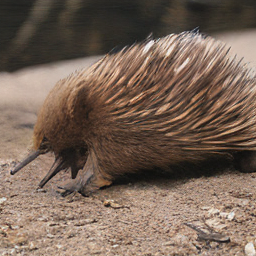
\includegraphics[width=\linewidth]{images/028102-class0102.png}
    \end{minipage}\hspace{0.01\textwidth}
    \begin{minipage}[t]{0.225\textwidth}
        \centering
        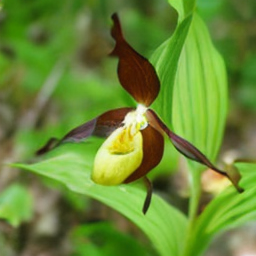
\includegraphics[width=\linewidth]{images/009986-class0986.png}
    \end{minipage}\hspace{0.01\textwidth}
    \begin{minipage}[t]{0.225\textwidth}
        \centering
        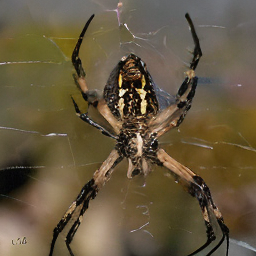
\includegraphics[width=\linewidth]{images/028072-class0072.png}
    \end{minipage}\hspace{0.01\textwidth}
    \begin{minipage}[t]{0.225\textwidth}
        \centering
        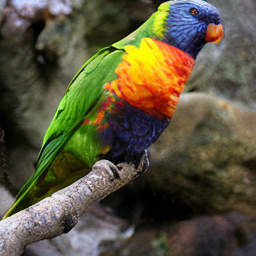
\includegraphics[width=\linewidth]{images/023090-class0090.png}
    \end{minipage}

    \vspace{1mm}

    \begin{minipage}[t]{0.225\textwidth}
        \centering
        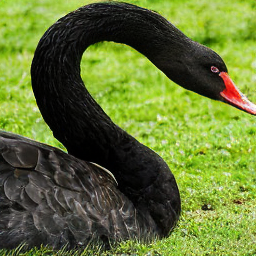
\includegraphics[width=\linewidth]{images/044100-class0100.png}
    \end{minipage}\hspace{0.01\textwidth}
    \begin{minipage}[t]{0.225\textwidth}
        \centering
        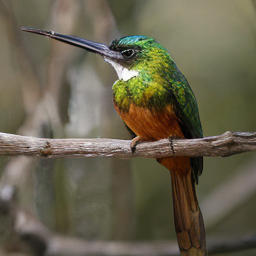
\includegraphics[width=\linewidth]{images/037095-class0095.png}
    \end{minipage}\hspace{0.01\textwidth}
    \begin{minipage}[t]{0.225\textwidth}
        \centering
        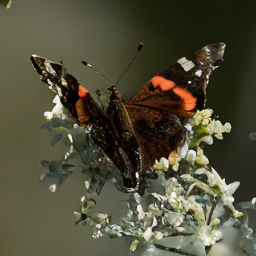
\includegraphics[width=\linewidth]{images/007321-class0321.png}
    \end{minipage}\hspace{0.01\textwidth}
    \begin{minipage}[t]{0.225\textwidth}
        \centering
        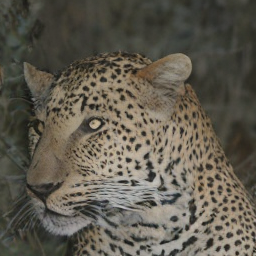
\includegraphics[width=\linewidth]{images/043288-class0288.png}
    \end{minipage}

    \vspace{1mm}

    \begin{minipage}[t]{0.225\textwidth}
        \centering
        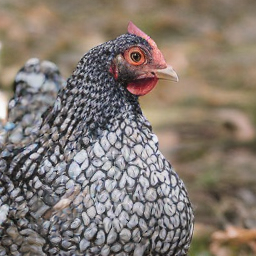
\includegraphics[width=\linewidth]{images/013008-class0008.png}
    \end{minipage}\hspace{0.01\textwidth}
    \begin{minipage}[t]{0.225\textwidth}
        \centering
        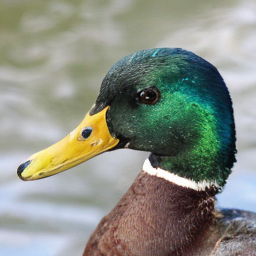
\includegraphics[width=\linewidth]{images/021097-class0097.png}
    \end{minipage}\hspace{0.01\textwidth}
    \begin{minipage}[t]{0.225\textwidth}
        \centering
        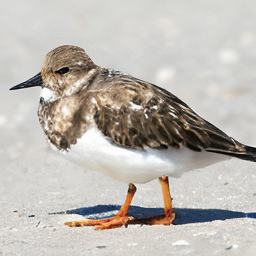
\includegraphics[width=\linewidth]{images/015139-class0139.png}
    \end{minipage}\hspace{0.01\textwidth}
    \begin{minipage}[t]{0.225\textwidth}
        \centering
        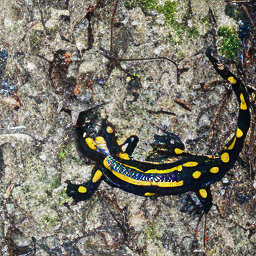
\includegraphics[width=\linewidth]{images/024025-class0025.png}
    \end{minipage}

    \vspace{1mm}

    \begin{minipage}[t]{0.225\textwidth}
        \centering
        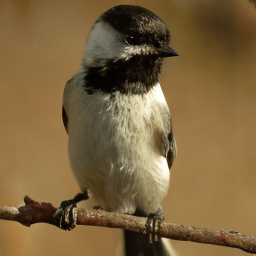
\includegraphics[width=\linewidth]{images/047019-class0019.png}
    \end{minipage}\hspace{0.01\textwidth}
    \begin{minipage}[t]{0.225\textwidth}
        \centering
        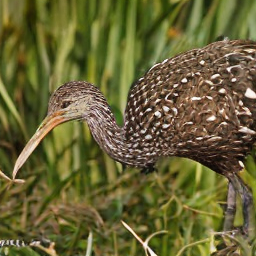
\includegraphics[width=\linewidth]{images/005135-class0135.png}
    \end{minipage}\hspace{0.01\textwidth}
    \begin{minipage}[t]{0.225\textwidth}
        \centering
        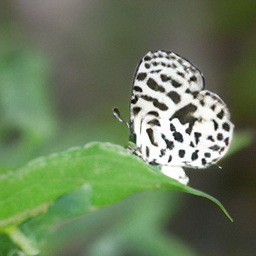
\includegraphics[width=\linewidth]{images/023326-class0326.png}
    \end{minipage}\hspace{0.01\textwidth}
    \begin{minipage}[t]{0.225\textwidth}
        \centering
        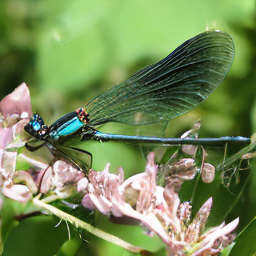
\includegraphics[width=\linewidth]{images/039320-class0320.png}
    \end{minipage}

    \vspace{1mm}

    \begin{minipage}[t]{0.225\textwidth}
        \centering
        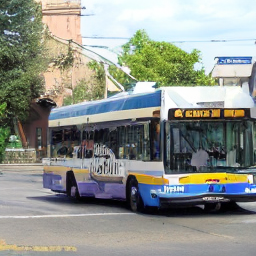
\includegraphics[width=\linewidth]{images/030874-class0874.png}
    \end{minipage}\hspace{0.01\textwidth}
    \begin{minipage}[t]{0.225\textwidth}
        \centering
        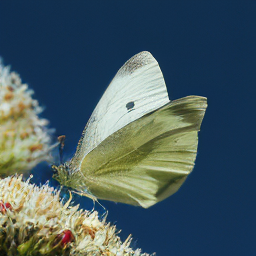
\includegraphics[width=\linewidth]{images/000324-class0324.png}
    \end{minipage}\hspace{0.01\textwidth}
    \begin{minipage}[t]{0.225\textwidth}
        \centering
        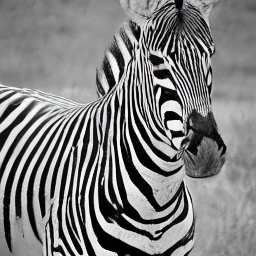
\includegraphics[width=\linewidth]{images/026340-class0340.png}
    \end{minipage}\hspace{0.01\textwidth}
    \begin{minipage}[t]{0.225\textwidth}
        \centering
        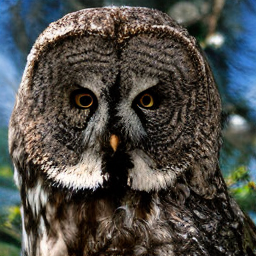
\includegraphics[width=\linewidth]{images/010024-class0024.png}
    \end{minipage}
    \caption[نمونه‌های تصویری \lr{DuoDiT-200}]{نمونه‌های تصویری تولیدشده توسط \lr{DuoDiT-200} روی کلاس‌های مختلف \lr{ImageNet}.}
    \label{fig:duodit_visual_results}
\end{figure}

\section{مطالعه انسانی}
برای تکمیل معیارهای خودکار، یک مطالعه انسانی میان نمونه‌های \lr{DuoDiT} و \lr{LightningDiT} انجام شده است. این مطالعه روی کلاس‌هایی از \lr{Mini-ImageNet}، به عنوان زیرمجموعه‌ای فشرده از \lr{ImageNet}، اجرا شده و شامل ۱۳ شرکت‌کننده است \cite{imagenet15russakovsky}. هر شرکت‌کننده ۳۰۰ مقایسه زوجی انجام داده و در مجموع ۳۹۰۰ پاسخ ثبت شده است.

\begin{table}[htbp]
    \centering
    \caption[نتایج مطالعه ترجیح انسانی]{نتایج مطالعه ترجیح انسانی برای مقایسه نمونه‌های \lr{DuoDiT} و \lr{LightningDiT}.}
    \label{tab:user_study_results}
    \begin{latin}
    \footnotesize
    \resizebox{\textwidth}{!}{%
    \begin{tabular}{ccccc}
        \hline
        \textbf{DuoDiT} & \textbf{LightningDiT} & \textbf{Tie} & \textbf{Total} & \textbf{DuoDiT Pref.} \\
        \hline
        1593 (40.85\%) & 1398 (35.85\%) & 909 (23.31\%) & 3900 & 53.26\% \\
        \hline
    \end{tabular}%
    }
    \end{latin}
    \begin{minipage}{0.96\linewidth}
        \footnotesize
        مقدار \lr{DuoDiT Pref.} از مقایسه‌های غیرمساوی محاسبه شده است؛ یعنی نسبت انتخاب‌های \lr{DuoDiT} به مجموع انتخاب‌های \lr{DuoDiT} و \lr{LightningDiT}.
    \end{minipage}
\end{table}

نتایج جدول \ref{tab:user_study_results} نشان می‌دهد با وجود برتری \lr{LightningDiT} در \lr{FID} کلی، نمونه‌های \lr{DuoDiT} در قضاوت انسانی سهم بیشتری از انتخاب‌های غیرمساوی را به دست آورده‌اند. این اختلاف با نتیجه \lr{LPIPS-Mean} همسو است و نشان می‌دهد شاخه وضوح‌بالا می‌تواند روی ویژگی‌هایی اثر بگذارد که در ادراک انسانی مهم هستند.

\section{هزینه محاسباتی و کارایی پارامتری}
جدول \ref{tab:compute_finediffusion} هزینه محاسباتی \lr{DuoDiT-200} را با \lr{FineDiffusion} مقایسه می‌کند. \lr{FineDiffusion} تعداد پارامتر آموزش‌پذیر کمتری دارد، اما در تنظیم پروفایل‌شده زمان هر دوره و مصرف حافظه بیشتری ثبت کرده است. در مقابل، \lr{DuoDiT-200} با \lr{17.95M} پارامتر آموزش‌پذیر، زمان هر دوره \lr{13m} و مصرف حافظه اوج \lr{2.91GB} را نشان می‌دهد.

\begin{table}[htbp]
    \centering
    \caption[مقایسه هزینه محاسباتی]{مقایسه هزینه محاسباتی و حافظه‌ای \lr{DuoDiT} و \lr{FineDiffusion} در تولید $256 \times 256$ \cite{Pan2024FineDiffusion}.}
    \label{tab:compute_finediffusion}
    \begin{latin}
    \footnotesize
    \resizebox{\textwidth}{!}{%
    \begin{tabular}{lccccc}
        \hline
        \textbf{Method} & \textbf{GFLOPs} & \textbf{Params} & \textbf{Trainable} & \textbf{Time/Epoch} & \textbf{VRAM} \\
        \hline
        DuoDiT-200 & 267.10 & 690.39M & 17.95M & 13m & 2.91GB \\
        FineDiffusion & 228.84 & 685.64M & 12.15M & 22m & 3.19GB \\
        \hline
    \end{tabular}%
    }
    \end{latin}
\end{table}

\section{مطالعات حذفی}
مطالعات حذفی برای جدا کردن اثر انتخاب‌های معماری انجام شده‌اند. این بخش شامل نتایج مربوط به راهبردهای تجمیع ویژگی، عمق شاخه دوم و نقش استفاده از ویژگی‌های \lr{ViT} و ضریب \lr{CFG} است. نتایج تجمیع ویژگی در سناریوی کنترل‌شده پنج‌کلاس ۹۷۲ تا ۹۷۶ گزارش شده‌اند تا اثر مکانیزم توکن کلاس محلی به‌صورت مستقیم با روش‌های ساده‌تر مقایسه شود.

\subsection{راهبردهای تجمیع ویژگی}
جدول \ref{tab:ablation_pooling} نشان می‌دهد که توکن کلاس محلی در مقایسه با میانگین‌گیری، بیشینه‌گیری و پروجکشن خطی بهترین مقدار را در هر سه معیار به دست می‌آورد. این نتیجه با انگیزه معماری سازگار است: تجمیع ثابت، همه نواحی مکانی را با قاعده یکسان خلاصه می‌کند، در حالی که توکن کلاس محلی از مکانیزم خود توجه برای استخراج محتوا-آگاه اطلاعات هر گروه چهار توکنی استفاده می‌کند.

\begin{table}[htbp]
    \centering
    \caption[مطالعه حذفی راهبردهای تجمیع]{مطالعه حذفی راهبردهای تجمیع برای هم‌تراز کردن توکن‌های شاخه دوم با شبکه توکنی \lr{DiT}.}
    \label{tab:ablation_pooling}
    \begin{latin}
    \begin{tabular}{lccc}
        \hline
        \textbf{Strategy} & \textbf{FID} ($\downarrow$) & \textbf{KID} ($\downarrow$) & \textbf{LPIPS-Mean} ($\downarrow$) \\
        \hline
        Average Pooling & 142.31 & 0.0452 & 0.7489 \\
        Max Pooling & 140.85 & 0.0438 & 0.7412 \\
        Linear Projection & 138.92 & 0.0415 & 0.7352 \\
        Local CLS Token & \textbf{135.78} & \textbf{0.0396} & \textbf{0.7018} \\
        \hline
    \end{tabular}
    \end{latin}
\end{table}

\subsection{عمق شاخه دوم}
جدول \ref{tab:ablation_blocks} هزینه اضافه کردن بلوک‌های بیشتر در شاخه دوم را نشان می‌دهد. افزایش عمق از یک بلوک به دو و چهار بلوک، \lr{GFLOPs}، زمان هر دوره و مصرف حافظه را افزایش می‌دهد. بنابراین تنظیم یک بلوک، نقطه تعادل مناسبی میان ظرفیت محلی و هزینه محاسباتی فراهم می‌کند.

\begin{table}[htbp]
    \centering
    \caption[مطالعه حذفی عمق شاخه دوم]{مطالعه حذفی عمق شاخه دوم از نظر محاسبات، زمان و حافظه.}
    \label{tab:ablation_blocks}
    \begin{latin}
    \begin{tabular}{lccc}
        \hline
        \textbf{Variant} & \textbf{GFLOPs} & \textbf{Time/Epoch} & \textbf{VRAM} \\
        \hline
        1 block & 267.10 & 13mins & 2.91GB \\
        2 blocks & 299.32 & 15mins & 2.99GB \\
        4 blocks & 363.75 & 26mins & 3.15GB \\
        \hline
    \end{tabular}
    \end{latin}
\end{table}

\subsection{ویژگی‌های شاخه دوم و ضریب \lr{CFG}}
جدول \ref{tab:ablation_vit} دو نوع تحلیل را نشان می‌دهد. در بخش نخست، استفاده از ویژگی‌های بلوک \lr{ViT} نسبت به اتصال ساده عملکرد کمی بهتری ثبت می‌کند. در بخش دوم، اثر ضریب \lr{CFG} بررسی شده است. باید توجه داشت که \lr{CFG} بخشی از معماری آموزش‌پذیر \lr{DuoDiT} نیست، بلکه ابرپارامتر مرحله نمونه‌برداری است؛ بنابراین تغییر آن مسیر حذف نویز و شدت شرط‌گذاری را تغییر می‌دهد، اما تعداد پارامترها یا ساختار شاخه دوم را عوض نمی‌کند.

در این تنظیم حذفی، ضریب \lr{CFG=1.0} بهترین \lr{FID} و \lr{KID} را دارد. افزایش ضریب به \lr{2.0} مقدار \lr{FID} را از \lr{210.3986} به \lr{215.7946} و مقدار \lr{KID} را از \lr{0.04142} به \lr{0.05030} افزایش می‌دهد. افزایش بیشتر ضریب به \lr{4.0} افت شدیدتری ایجاد می‌کند و \lr{FID} به \lr{230.0816} و \lr{KID} به \lr{0.06270} می‌رسد. این الگو نشان می‌دهد در این آزمایش، تقویت بیش از حد شرط باعث دور شدن نمونه‌ها از توزیع مرجع می‌شود. با این حال، تنظیم نهایی پایان‌نامه برای ارزیابی اصلی از \lr{CFG=1.5} استفاده می‌کند تا میان وفاداری شرطی و تنوع نمونه‌ها تعادل حفظ شود.

\begin{table}[htbp]
    \centering
    \caption[مطالعه حذفی شاخه دوم و \lr{CFG}]{مطالعه حذفی استفاده از ویژگی‌های شاخه دوم و مقدار ضریب \lr{CFG}.}
    \label{tab:ablation_vit}
    \begin{latin}
    \begin{tabular}{lcc}
        \hline
        \textbf{Variant} & \textbf{FID} ($\downarrow$) & \textbf{KID} ($\downarrow$) \\
        \hline
        Skip Connection & 216.7914 & 0.0512 \\
        ViT block features & 215.7946 & 0.0503 \\
        \hline
        CFG = 1.0 & 210.3986 & 0.04142 \\
        CFG = 2.0 & 215.7946 & 0.05030 \\
        CFG = 4.0 & 230.0816 & 0.06270 \\
        \hline
    \end{tabular}
    \end{latin}
\end{table}

تفسیر این نتیجه با نقش نظری \lr{CFG} سازگار است. ضریب بزرگ‌تر معمولاً نمونه‌ها را از نظر معنایی به کلاس خواسته‌شده نزدیک‌تر می‌کند و می‌تواند برای ارزیابی انسانی یا تولید نمونه‌های واضح‌تر مفید باشد، اما همین تقویت ممکن است تنوع درون‌کلاسی را کم کند. معیارهایی مانند \lr{FID} و \lr{KID} فقط وضوح یا تشخیص‌پذیری کلاس را اندازه نمی‌گیرند، بلکه شباهت توزیع تصاویر تولیدی به توزیع واقعی را نیز می‌سنجند. بنابراین، اگر \lr{CFG} خیلی زیاد باشد، خروجی‌ها ممکن است از نظر شرطی قوی‌تر اما از نظر توزیعی کم‌تنوع‌تر شوند و امتیاز بدتری بگیرند. به همین دلیل، در تحلیل نتایج این پایان‌نامه، \lr{CFG} به‌عنوان عامل کنترل‌کننده نمونه‌برداری از اثر معماری شاخه دوم جدا تفسیر می‌شود.

\section{بحث}
نتایج این فصل نشان می‌دهد \lr{DuoDiT} یک مسیر مکمل برای تنظیم دقیق پارامتر-کارای \lr{DiT} فراهم می‌کند. بدنه منجمد \lr{DiT} ساختار معنایی و دانش تولیدی پیش‌آموزش‌دیده را حفظ می‌کند، در حالی که شاخه دوم با اندازه پچ کوچک‌تر ویژگی‌های محلی بیشتری را در اختیار مدل قرار می‌دهد. مکانیزم توکن کلاس محلی نیز این ویژگی‌های ریزدانه را بدون افزایش طول توالی بدنه اصلی، به شبکه توکنی \lr{DiT} منتقل می‌کند.

برتری \lr{DuoDiT-200} در \lr{KID} و \lr{LPIPS-Mean} نشان می‌دهد اثر شاخه دوم بیشتر در شباهت توزیعی پایدار و کیفیت ادراکی ظاهر می‌شود. از سوی دیگر، مقدار \lr{FID} مدل همچنان از \lr{LightningDiT} بالاتر است؛ بنابراین ادعای این پایان‌نامه جایگزینی کامل روش‌های آموزش بزرگ‌مقیاس نیست، بلکه ارائه یک مسیر سبک برای تقویت مدل منجمد است. محدودیت اصلی آن است که شاخه محلی در برخی نمونه‌های دارای مرزهای مبهم یا بافت‌های بسیار متراکم ممکن است ساختار محلی نادرست را نیز تقویت کند. بررسی شرط‌گذاری اختیاری \lr{FiLM} و طراحی چندمقیاسی شاخه دوم می‌تواند در پژوهش‌های آینده برای کاهش این خطاها مطالعه شود.
